\documentclass[tikz,border=4pt]{standalone}
% Estilo común de los diagramas de bloques (se usa con \input en cada standalone)
\usepackage[defaultsans,scale=0.92]{lato}
\usepackage{libertinust1math}
\usepackage{xcolor,amsmath}
\usepackage{tikz}
\usetikzlibrary{positioning,arrows.meta,calc,shapes.geometric}
\usepackage{../../notacion}
\definecolor{ctrlazul}{HTML}{1E5AA8}\definecolor{ctrlnoche}{HTML}{14213D}
\definecolor{ctrlcoral}{HTML}{D1495B}\definecolor{ctrlverde}{HTML}{2A9D8F}
\definecolor{ctrlambar}{HTML}{E09F3E}\definecolor{ctrlgris}{HTML}{5C677D}
\definecolor{ctrlvioleta}{HTML}{6C4AB6}\definecolor{ctrlteal}{HTML}{0F7173}
\tikzset{
  >={Stealth[length=2.4mm]}, every node/.style={font=\small},
  bloque/.style={draw=ctrlnoche,fill=ctrlazul!7,thick,rounded corners=1.5pt,minimum height=9mm,minimum width=13mm,inner sep=4pt},
  suma/.style={draw=ctrlnoche,thick,circle,inner sep=0pt,minimum size=6mm},
  senal/.style={->,thick,draw=ctrlnoche},
  rot/.style={font=\footnotesize,text=ctrlgris},
}

\begin{document}
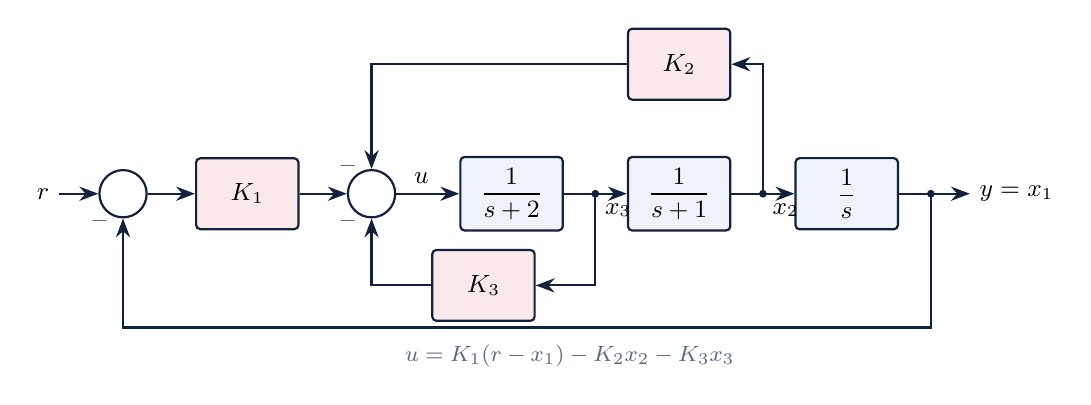
\begin{tikzpicture}[node distance=8mm]
  \node (r) {$r$}; \node[suma,right=5mm of r] (S1) {};
  \node[bloque,right=6mm of S1,fill=ctrlcoral!12] (K1) {$K_1$};
  \node[suma,right=6mm of K1] (S2) {};
  \node[bloque,right=8mm of S2] (G1) {$\dfrac{1}{s+2}$};
  \node[bloque,right=8mm of G1] (G2) {$\dfrac{1}{s+1}$};
  \node[bloque,right=8mm of G2] (G3) {$\dfrac{1}{s}$};
  \node[right=9mm of G3] (y) {$y=x_1$};
  \coordinate (a) at ($(G1.east)!0.5!(G2.west)$); \coordinate (b) at ($(G2.east)!0.5!(G3.west)$);
  \coordinate (c) at ($(G3.east)!0.45!(y.west)$);
  \node[bloque,below=7mm of G1,fill=ctrlcoral!12] (K3) at ($(a)!0.5!(S2)$) {$K_3$};
  \node[bloque,above=7mm of G2,fill=ctrlcoral!12] (K2) {$K_2$};
  \draw[senal] (r)--(S1); \draw[senal] (S1)--(K1); \draw[senal] (K1)--(S2); \draw[senal] (S2)--node[above,pos=0.4]{$u$}(G1);
  \draw[senal] (G1)--(G2); \draw[senal] (G2)--(G3); \draw[senal] (G3)--(y);
  \fill[ctrlnoche] (a) circle (1.4pt) (b) circle (1.4pt) (c) circle (1.4pt);
  \node[below right] at (a) {$x_3$}; \node[below right] at (b) {$x_2$};
  \draw[senal] (a)|-(K3); \draw[senal] (K3)-|(S2);
  \draw[senal] (b)|-(K2); \draw[senal] (K2)-|(S2);
  \draw[senal] (c)--++(0,-17mm)-|(S1);
  \node[rot] at ($(S1)+(-3mm,-3.5mm)$) {$-$}; \node[rot] at ($(S2)+(-3mm,-3.5mm)$) {$-$}; \node[rot] at ($(S2)+(-3mm,3.5mm)$) {$-$};
  \node[rot,anchor=north] at ($(S1)!0.5!(y)+(0,-18mm)$) {$u=K_1(r-x_1)-K_2x_2-K_3x_3$};
\end{tikzpicture}
\end{document}
